% --- Distillation training: soft targets, temperature, and loss ---
\begin{frame}{Distillation: Soft Targets}
  \textbf{\textcolor{blue}{While training, our confidence in the labels must be high.}}\\[0.8em]
  Otherwise the data would not be present in the training set.\\[1em]
  \begin{columns}[T,onlytextwidth]
    \column{0.49\textwidth}
      \small
      For example: \\[0.7em]
      \texttt{This is a Dog}
      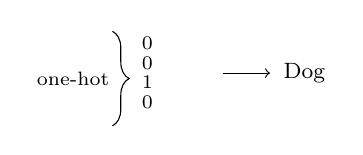
\begin{tikzpicture}[baseline={(0,0)}]
        % Draw brace + label for one-hot
        \draw[decorate,decoration={brace,amplitude=6pt,mirror}] (0,-0.2) -- (0,1) node[midway,xshift=-0.5cm] {\scriptsize one-hot};
        % One-hot vector
        \node[anchor=west] at (0.25,0.85) {\scriptsize 0};
        \node[anchor=west] at (0.25,0.60) {\scriptsize 0};
        \node[anchor=west] at (0.25,0.35) {\scriptsize 1};
        \node[anchor=west] at (0.25,0.10) {\scriptsize 0};
        % Arrow to "Dog"
        \draw[->] (1.4,0.47) -- (2,0.47);
        \node[anchor=west] at (2.05,0.47) {\footnotesize Dog};
      \end{tikzpicture}
    \column{0.48\textwidth}
      \centering
      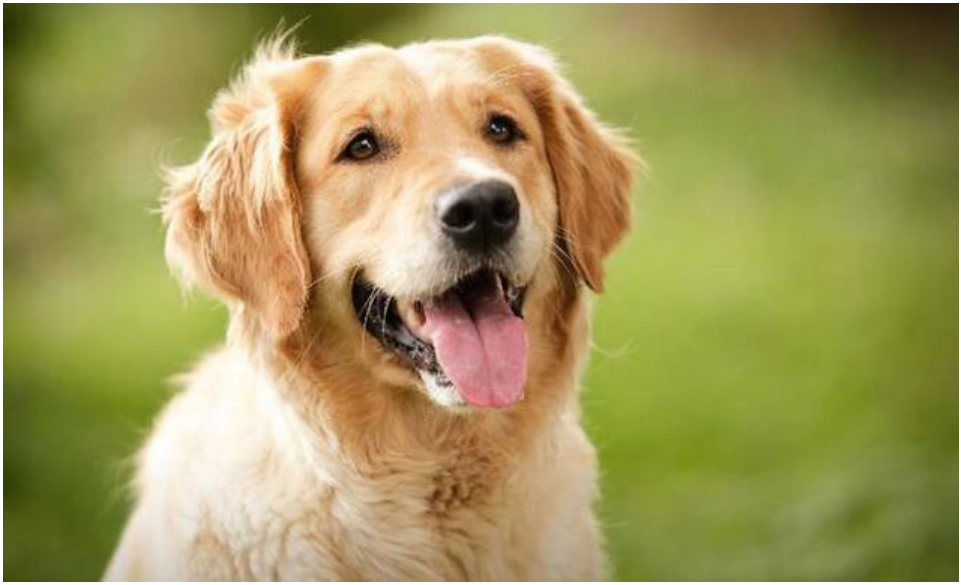
\includegraphics[width=\linewidth,height=0.5\textheight,keepaspectratio]{images/inference-optimisation/distillation_golden_retriever_teacher.png}\\[0.25em]
      {\scriptsize Photo: Harvard IACS AC215, Lecture 11, \href{https://harvard-iacs.github.io/2024-AC215/assets/lectures/lecture11/L11_compression_techniques.pdf}{p.~14}.}
  \end{columns}
  \vspace{0.4em}
\end{frame}


\begin{frame}{Distillation: Soft Targets}
  \textbf{\textcolor{blue}{While training, our confidence in the labels must be high.}}\\[0.8em]
  Otherwise the data would not be present in the training set.\\[1em]
  \begin{columns}[T,onlytextwidth]
    \column{0.49\textwidth}
      \small
      For example: \\[0.7em]
      \texttt{This is also a Dog}
      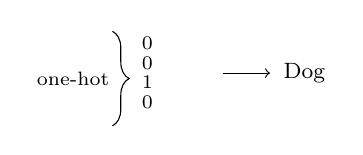
\begin{tikzpicture}[baseline={(0,0)}]
        % Draw brace + label for one-hot
        \draw[decorate,decoration={brace,amplitude=6pt,mirror}] (0,-0.2) -- (0,1) node[midway,xshift=-0.5cm] {\scriptsize one-hot};
        % One-hot vector
        \node[anchor=west] at (0.25,0.85) {\scriptsize 0};
        \node[anchor=west] at (0.25,0.60) {\scriptsize 0};
        \node[anchor=west] at (0.25,0.35) {\scriptsize 1};
        \node[anchor=west] at (0.25,0.10) {\scriptsize 0};
        % Arrow to "Dog"
        \draw[->] (1.4,0.47) -- (2,0.47);
        \node[anchor=west] at (2.05,0.47) {\footnotesize Dog};
      \end{tikzpicture}
    \column{0.48\textwidth}
      \centering
      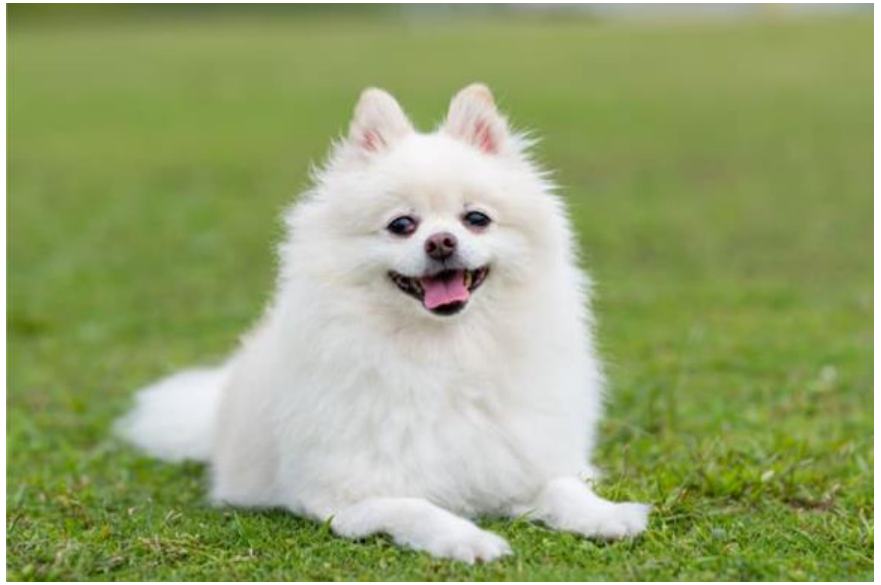
\includegraphics[width=\linewidth,height=0.5\textheight,keepaspectratio]{images/inference-optimisation/distillation_pomeranian_student.png}\\[0.25em]
      {\scriptsize Photo: Harvard IACS AC215, Lecture 11, \href{https://harvard-iacs.github.io/2024-AC215/assets/lectures/lecture11/L11_compression_techniques.pdf}{p.~15}.}
  \end{columns}
  \vspace{0.4em}
\end{frame}

\begin{frame}{Distillation: Soft Targets}
  \textbf{\textcolor{blue}{While training, our confidence in the labels must be high.}}\\[0.8em]
  Otherwise the data would not be present in the training set.\\[1em]
  \begin{columns}[T,onlytextwidth]
    \column{0.49\textwidth}
      \small
      For example: \\[0.7em]
      \texttt{This is a Cat}
      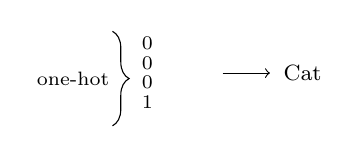
\begin{tikzpicture}[baseline={(0,0)}]
        % Draw brace + label for one-hot
        \draw[decorate,decoration={brace,amplitude=6pt,mirror}] (0,-0.2) -- (0,1) node[midway,xshift=-0.5cm] {\scriptsize one-hot};
        % One-hot vector. The 1 sits in the fourth slot: the class order used
        % throughout this section is (cow, car, dog, cat), so a cat is not slot 3.
        \node[anchor=west] at (0.25,0.85) {\scriptsize 0};
        \node[anchor=west] at (0.25,0.60) {\scriptsize 0};
        \node[anchor=west] at (0.25,0.35) {\scriptsize 0};
        \node[anchor=west] at (0.25,0.10) {\scriptsize 1};
        % Arrow to the active class
        \draw[->] (1.4,0.47) -- (2,0.47);
        \node[anchor=west] at (2.05,0.47) {\footnotesize Cat};
      \end{tikzpicture}
    \column{0.48\textwidth}
      \centering
      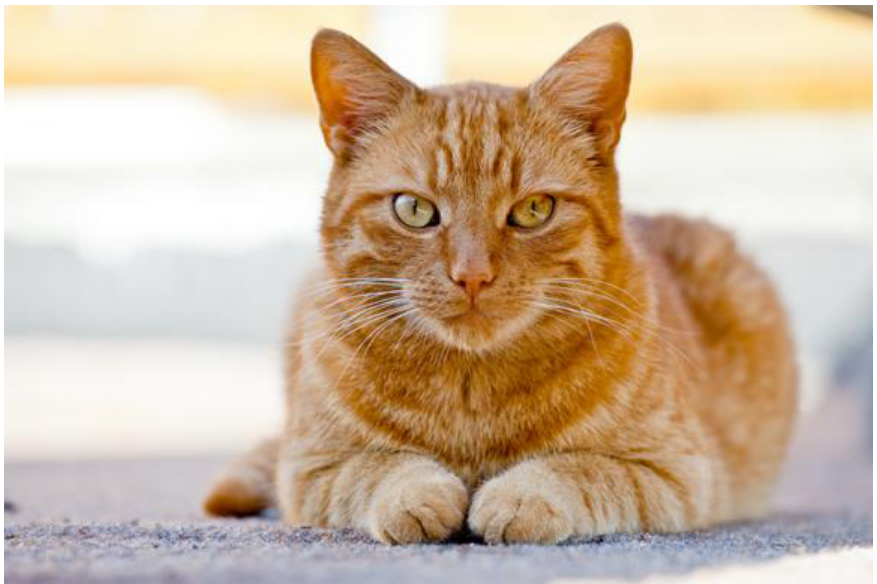
\includegraphics[width=\linewidth,height=0.5\textheight,keepaspectratio]{images/inference-optimisation/distillation_orange_cat_analogy.png}\\[0.25em]
      {\scriptsize Photo: Harvard IACS AC215, Lecture 11, \href{https://harvard-iacs.github.io/2024-AC215/assets/lectures/lecture11/L11_compression_techniques.pdf}{p.~17}.}
  \end{columns}
  \vspace{0.4em}
\end{frame}

\begin{frame}{Distillation: Soft targets}
  \begin{columns}[T,onlytextwidth]
    \column{0.55\textwidth}
      \vspace{0.5em}
      \textbf{What about this example?}\\[1.2em]
      \texttt{This is a \ldots}
      % Mass is split across slots 3 and 4, i.e. dog and cat in the (cow, car,
      % dog, cat) ordering used by the tables that follow.
      \[
        \begin{pmatrix}
          0 \\
          0 \\
          0.5 \\
          0.5 \\
        \end{pmatrix}
      \]

    \column{0.44\textwidth}
      \centering
      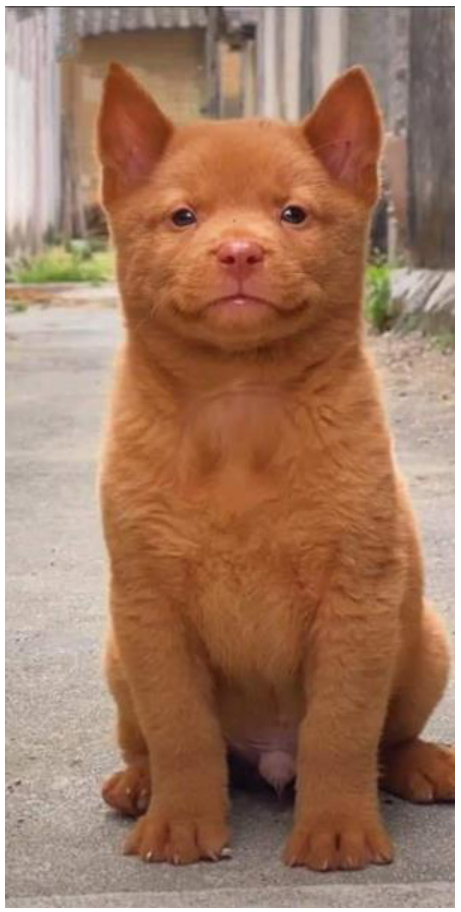
\includegraphics[width=0.78\linewidth,height=0.5\textheight,keepaspectratio]{images/inference-optimisation/distillation_brown_puppy_analogy.png}\\[0.2em]
      {\scriptsize Photo: Harvard IACS AC215, Lecture 11, \href{https://harvard-iacs.github.io/2024-AC215/assets/lectures/lecture11/L11_compression_techniques.pdf}{p.~19}.}
  \end{columns}
  \vspace{0.3em}
\end{frame}

\begin{frame}{Distillation: Soft targets}
  \begin{columns}[T,onlytextwidth]
    \column{0.55\textwidth}
      \vspace{0.5em}
      In the real world, the distinction is never that clear.

      Ideally, the \href{https://en.wikipedia.org/wiki/Soft_target}{training labels must be soft}, to learn about the nuanced relations across the elements of the dataset.

    \column{0.44\textwidth}
      \centering
      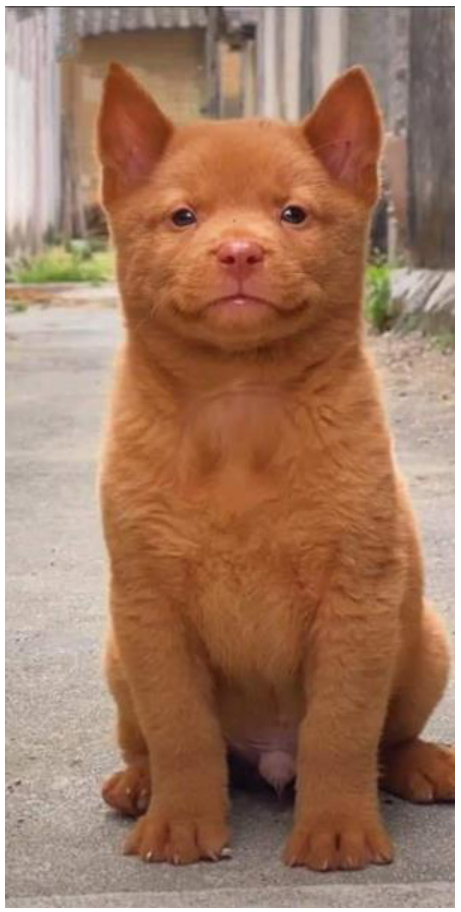
\includegraphics[width=0.78\linewidth,height=0.5\textheight,keepaspectratio]{images/inference-optimisation/distillation_brown_puppy_analogy.png}\\[0.2em]
      {\scriptsize Photo: Harvard IACS AC215, Lecture 11, \href{https://harvard-iacs.github.io/2024-AC215/assets/lectures/lecture11/L11_compression_techniques.pdf}{p.~20}.}
  \end{columns}
  \vspace{0.3em}
\end{frame}

\begin{frame}{Distillation: Teacher -- Student}
  \begin{columns}[T,onlytextwidth]
    \column{0.52\textwidth}
      The teacher shows the student the \textcolor{blue}{relations} between the different classes, based on what it \textcolor{blue}{learned} during its training stage.

      \vspace{0.6em}
      From a dataset containing the original categories, the teacher outputs the \textcolor{blue}{normalized probabilities} for each example.

    \column{0.46\textwidth}
      \centering
      \setlength{\tabcolsep}{0.45em}
      \renewcommand{\arraystretch}{1.22}
      \begin{tabular}{c|cccc}
        & \footnotesize cow & \footnotesize car & \footnotesize dog & \footnotesize cat \\
        \hline
        \footnotesize Original labels & $0$ & $1$ & $0$ & $0$ \\
        \footnotesize Probabilities & $10^{-6}$ & $0.9$ & $0.1$ & $10^{-9}$ \\
      \end{tabular}
 
      \vspace{0.6em}

      {\scriptsize
        Adapted from:\par
        Geoffrey Hinton, Oriol Vinyals \& Jeff Dean, \href{https://arxiv.org/abs/1503.02531}{\textit{Distilling the Knowledge in a Neural Network}}
      }
  \end{columns}
\end{frame}

\begin{frame}{Distillation: Teacher -- Student (Softening with Temperature)}
  \begin{columns}[T,onlytextwidth]
    \column{0.52\textwidth}
      To enhance the student's learning, the teacher \textcolor{blue}{softens} its output $z$ even more.

      \vspace{0.7em}
      To do this, it introduces the softmax function with temperature $T$:

      \begin{align*}
        q_i = \frac{\exp\left(z_i / T\right)}{\sum\limits_j \exp\left(z_j / T\right)}
      \end{align*}

      \vspace{0.5em}
      {\footnotesize The softened row is the same logits $z$ pushed through this softmax at $T = 5$; like any softmax output, it still sums to $1$.}

      \vspace{0.5em}
      ``Soft'' targets allow the student to learn the teacher's implicit knowledge about class similarities.

    \column{0.46\textwidth}
      \centering
      % Tight columns: the three-row table has to fit a 0.46\textwidth column.
      \setlength{\tabcolsep}{0.25em}
      \renewcommand{\arraystretch}{1.1}
      \begin{tabular}{c|cccc}
        & \footnotesize cow & \footnotesize car & \footnotesize dog & \footnotesize cat \\
        \hline
        \footnotesize Original labels & $0$ & $1$ & $0$ & $0$ \\
        \footnotesize Softmax probabilities & $10^{-6}$ & $0.9$ & $0.1$ & $10^{-9}$ \\
        \footnotesize Softened, $T{=}5$ & $0.04$ & $0.58$ & $0.37$ & $0.01$
      \end{tabular}

      \vspace{0.75em}
      {\footnotesize
        Adapted from:\par
        Geoffrey Hinton, Oriol Vinyals \& Jeff Dean, \href{https://arxiv.org/abs/1503.02531}{\textit{Distilling the Knowledge in a Neural Network}}
      }
  \end{columns}
\end{frame}

\begin{frame}{Distillation: Teacher -- Student (Softening with Temperature)}
  \begin{columns}[T,onlytextwidth]
    \column{0.52\textwidth}
      A high value of $T$ will dilute the information contained in the probabilities.
      \begin{itemize}
        \item The standard softmax is recovered for $T{=}1$.
        \item For $T{>}1$, the probabilities are softened. Typical values range between $2$ and $5$.
        \item For $T{<}1$, it approaches to the original one-hot labels.
      \end{itemize}
 

    \column{0.46\textwidth}
      \centering
      % Tight columns: the three-row table has to fit a 0.46\textwidth column.
      \setlength{\tabcolsep}{0.25em}
      \renewcommand{\arraystretch}{1.1}
      \begin{tabular}{c|cccc}
        & \footnotesize cow & \footnotesize car & \footnotesize dog & \footnotesize cat \\
        \hline
        \footnotesize Original labels & $0$ & $1$ & $0$ & $0$ \\
        \footnotesize Softmax probabilities & $10^{-6}$ & $0.9$ & $0.1$ & $10^{-9}$ \\
        \footnotesize Softened, $T{=}5$ & $0.04$ & $0.58$ & $0.37$ & $0.01$
      \end{tabular}

      \vspace{0.75em}
      {\footnotesize
        Adapted from:\par
        Geoffrey Hinton, Oriol Vinyals \& Jeff Dean, \href{https://arxiv.org/abs/1503.02531}{\textit{Distilling the Knowledge in a Neural Network}}
      }
  \end{columns}
\end{frame}

\begin{frame}{Distillation: Teacher--Student Training}
  \begin{columns}[T,onlytextwidth]
    \column{0.47\textwidth}
      \vspace{0.5em}
      \begin{itemize}\itemsep0.7em
        \item The student is trained to both:
        \begin{itemize}
          \item Solve the original task (matching the hard/true labels).
          \item Replicate the softened probabilities (soft labels) from the teacher.
        \end{itemize}
        \item This allows the student to learn not only the correct answer, but also the teacher's representation of class similarities.
      \end{itemize}
    \column{0.53\textwidth}
      \centering
      \fbox{
        \parbox[c][4.2cm][c]{0.92\linewidth}{
          \centering
          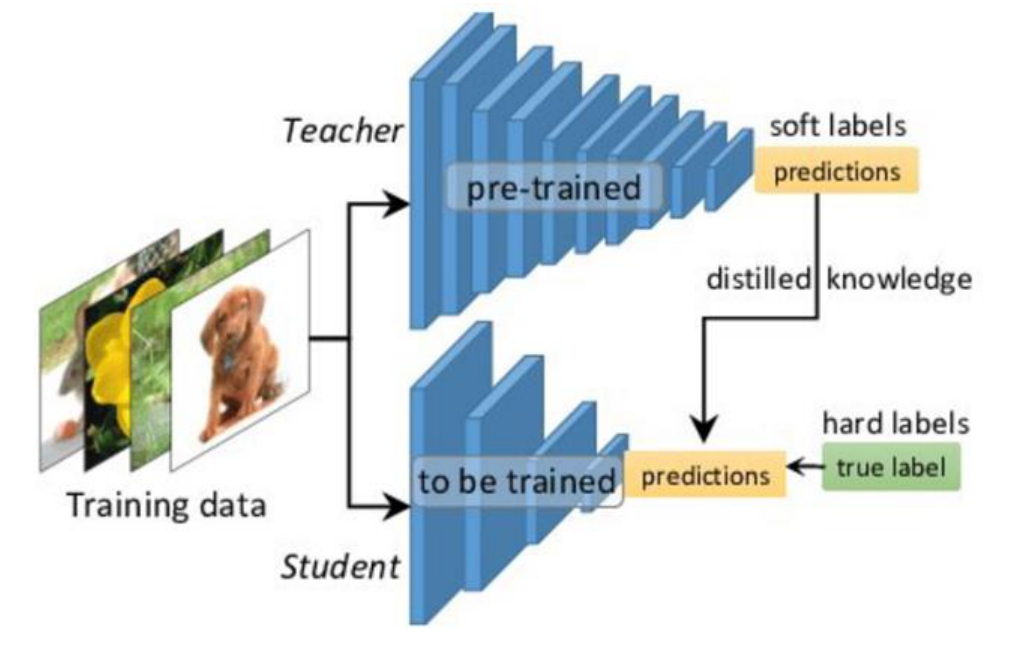
\includegraphics[width=0.78\linewidth,height=0.5\textheight,keepaspectratio]{images/inference-optimisation/distillation_teacher_student_soft_hard_labels.png}\\[0.2em]
          {\scriptsize Figure: Harvard IACS AC215, Lecture 11, \href{https://harvard-iacs.github.io/2024-AC215/assets/lectures/lecture11/L11_compression_techniques.pdf}{p.~25}; credited there to Hinton, Vinyals \& Dean, \textit{Dark Knowledge}.}
     
        }
      }
      \vspace{0.5em}

  \end{columns}
\end{frame}

\begin{frame}{Distillation: Teacher--Student Scenarios}
  \vspace{0.6em}
  \textbf{Scenario 1:}
  \begin{itemize}
    \item[] Train on the same data as the teacher model. \\
      {\scriptsize (DistilBERT was trained on this example.)}
  \end{itemize}
  \vspace{0.5em}
  \textbf{Scenario 2:}
  \begin{itemize}
    \item[] Train on a reduced dataset. This is usually done when you have the teacher model but not the original dataset or resources.
  \end{itemize}
  \vspace{1em}
\end{frame}

\begin{frame}{Distillation: Teacher--Student Loss}
  \begin{columns}[T,onlytextwidth]
    \column{0.54\textwidth}
      It minimizes the sum of two different cross-entropy functions:
      \begin{itemize}\itemsep0.35em
        \item One involving the original hard labels obtained using a softmax with $T = 1$.
        \item One involving the softened probabilities with $T > 1$.
        \item {\footnotesize The gradients of the soft-target term scale as $1/T^{2}$, so in practice that term is multiplied by $T^{2}$. Without it, raising $T$ would quietly shrink the distillation signal relative to the hard-label one.}
      \end{itemize}
    \column{0.42\textwidth}
      \centering
      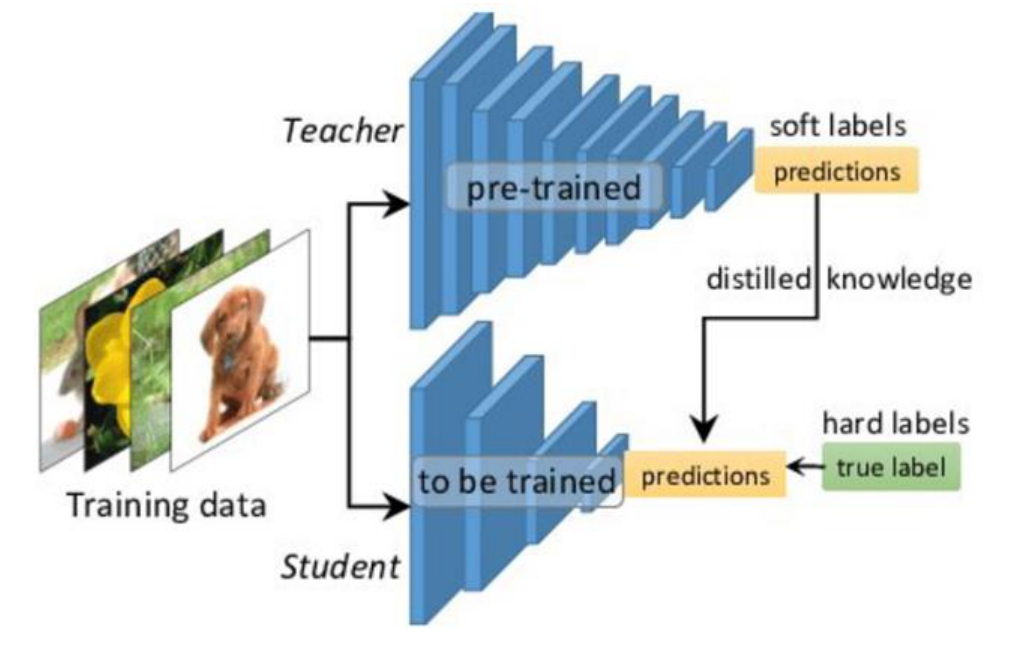
\includegraphics[width=0.98\linewidth,height=0.5\textheight,keepaspectratio]{images/inference-optimisation/distillation_teacher_student_soft_hard_labels.png}\\[0.2em]
      {\scriptsize Figure: Harvard IACS AC215, Lecture 11, \href{https://harvard-iacs.github.io/2024-AC215/assets/lectures/lecture11/L11_compression_techniques.pdf}{p.~25}; credited there to Hinton, Vinyals \& Dean, \textit{Dark Knowledge}.}
  \end{columns}
\end{frame}

\begin{frame}{Distillation: Teacher--Student}
  \centering
  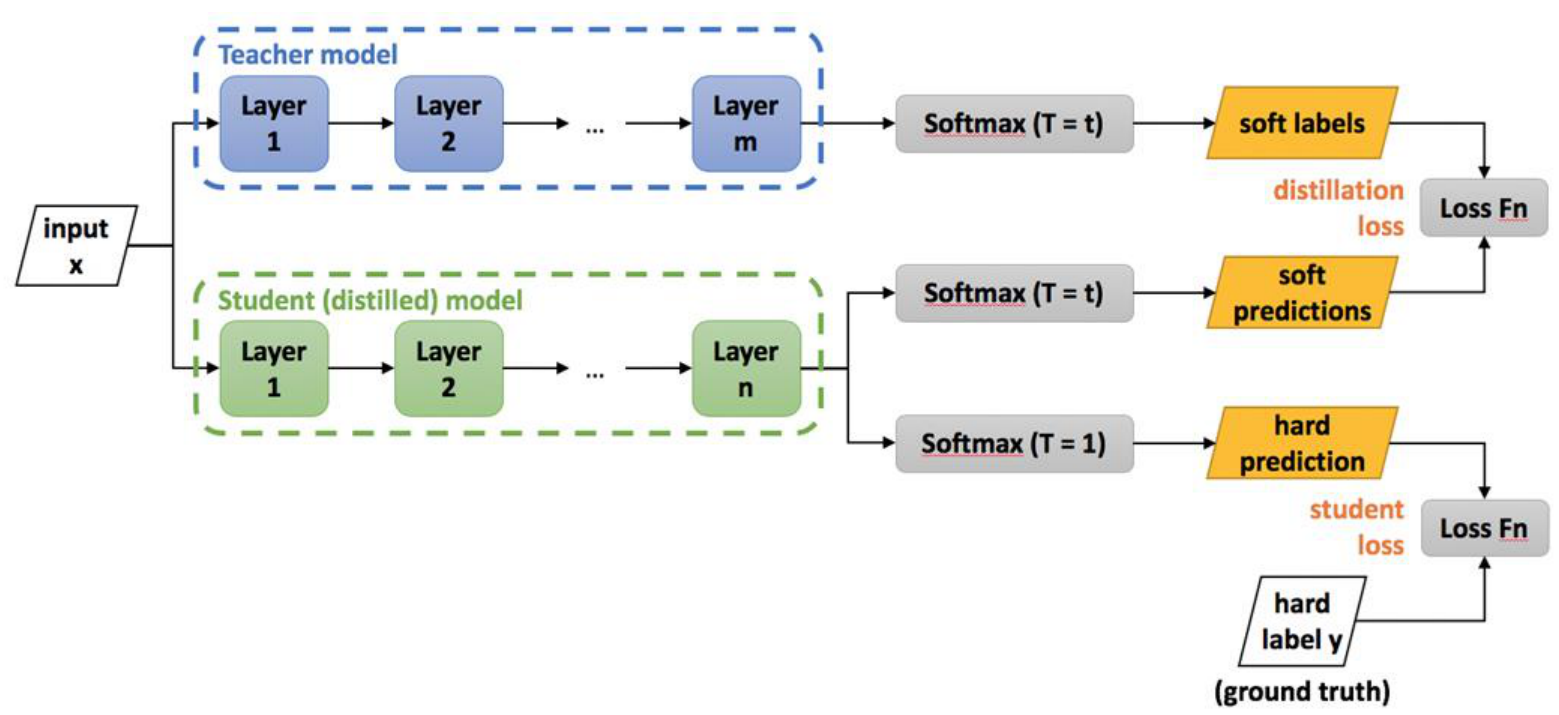
\includegraphics[width=0.97\linewidth,height=0.62\textheight,keepaspectratio]{images/inference-optimisation/distillation_softmax_temperature_loss_diagram.png}\\[0.3em]
  {\scriptsize Figure: Harvard IACS AC215, Lecture 11, \href{https://harvard-iacs.github.io/2024-AC215/assets/lectures/lecture11/L11_compression_techniques.pdf}{p.~28}. Temperature and loss scheme: Hinton, Vinyals \& Dean, \textit{Distilling the Knowledge in a Neural Network}.}
  \vspace{0.2em}
  \[
    L = \lambda L_{\mathrm{student}} + (1-\lambda) L_{\mathrm{distillation}}
  \]
\end{frame}

\begin{frame}{Distillation: Teacher--Student}
  \small
  \[
    L_\mathrm{Distillation} = -\sum_{k=1}^{K} p_T^k(x, T)\log\big(q_S^k(x, T)\big)
  \]
  \vspace{0.8em}

  In our example, for the example $n$ in the dataset:
  \[
    p_T(x, T) = [0.04,\ 0.58,\ 0.37,\ 0.01]
  \]

  And our predictions
  \[
    q_S(x, T) = [0.1,\ 0.45,\ 0.30,\ 0.15]
  \]

  The resulting loss value for this example is:
  \[
    -\Big[0.04 \log(0.1) + 0.58 \log(0.45) + 0.37 \log(0.30) + 0.01 \log(0.15)\Big] \approx 1.02
  \]
\end{frame}

\begin{frame}{Distilling Reasoning Traces}
  \begin{itemize}\footnotesize\itemsep0.45em
    \item Classic distillation transfers the teacher's \textbf{output distribution}: the student matches softened logits, one prediction at a time.
    \item For reasoning models the valuable signal is the \textbf{trace}: the chain of intermediate steps the teacher produces before its answer.
    \item \textbf{Recipe:} generate many problems' worth of full reasoning traces with a large reasoning model, filter for correct answers, then fine-tune the small model on the traces with plain supervised learning. No logits, no RL. The filter-on-correct-answers step is the idea behind STaR (Zelikman et al., 2022).
    \item DeepSeek distilled R1 traces into Qwen and Llama models from 1.5B to 70B this way, using 800k curated samples and supervised fine-tuning only; the distilled students beat much larger non-reasoning baselines on math and code benchmarks.
    \item The trade: trace distillation is far cheaper than running RL on the small model, but the student inherits the teacher's reasoning style, including its mistakes.
  \end{itemize}
  \vspace{0.2em}
  {\scriptsize DeepSeek-AI, ``DeepSeek-R1: Incentivizing Reasoning Capability in LLMs via Reinforcement Learning,'' \href{https://arxiv.org/abs/2501.12948}{arXiv:2501.12948}.}
\end{frame}
